\scanpage{54}
% E: text|upper left, instruction|Réécrit sans utiliser
\uline{\unsure{Réécrit|Récrit}} sans utiliser la position des arcs critiques, pour déterminer les signes de \(\varepsilon_{F'}(\deleted{\unsure{\alpha}}a')\), quand on connaît \deleted{\unsure{les signes}} \(\varepsilon_F(a)\).

\deleted{
% E: text|left upper, rejected proposition|Considérons l'ens V_F
\uline{Proposition}. Considérons l'ens \deleted{\unsure{de}} \(V_F\) (``\(\mathrm{vert}^4\)'') des sommets d'ordre 4 incidents à \(F\), et l'ens \(\sigma_a^{F'}(V_{F'})\) (où \(F'\) est la face incidente à \(F\) le long de le grand côté \(a\) de \(\delta F\)).

\deleted{Soit \unsure{\(\sigma_a(V_{F'})\)}} \unsure{les réunir dans décomposition} de \(\delta F\) en \deleted{\unsure{grands côtés}}\inserted{côtés} \unsure{considérés les} (fermés) \(\alpha\),
}

% E: text|left middle, new definition|Soit A_F a
Soit \(A_{F,a}=\unsure{A}\) la réunion des grands côtés en \(F\) qui sont telles que \(\sigma_a(\unsure{\alpha})\) est un grand côté de \(F'=\sigma_a(F)\) (NB \(a\) est un grand côté de \(F\)) Alors

% E: text|left lower, a|A est un arc
a) \(A\) est un arc sur \(\delta F\), soit \(B\) l'arc ``complémentaire''

\deleted{Alors} Considérons la subdivision de \(B\) en grands côtés (sommets verts clairs) et en ``grands côtés pour \(F'\)'' (sommets verts foncés). Alors le nb d'arêtes \(n_a(F)\) et \(n_a(F')\) qui interviennent est \unsure{compris} entre 3 et 5 --- les possibilités sont (\unsure{à un échange identique|à un échange} de \(F\) et \(F'\)) \(\unsure{(3,2)},\unsure{(3,3)},\unsure{(3,5)|(3,4)}\) \deleted{\unsure{Dans le cas particulier \(1)\ 2)\ 2)\)}} --- et dans tous les cas, c'est la face spéciale qui donne lieu à \unsure{3} arcs (ce qui suffit à le déterminer, quand on est dans le cas \(1^\circ\) ou \(3^\circ\)). De plus, on a

% E: text|right upper, b|Si alpha est une arête
b) Si \(\alpha\) est une\deleted{petite} arête de \(F\) dans \(A\), \deleted{\unsure{alors}} et \(\alpha\ne a\), on a \(\varepsilon_{F'}(\unsure{a|\alpha})=\varepsilon_F(\unsure{a|\alpha})\)

\([\mathrm{NB}\) si \(\alpha=a\), on a \(\varepsilon_{F'}(a)=-\varepsilon_F(a)]\)

% E: text|right upper-middle, c|On a les trois cas suivants
c) On a les \deleted{\unsure{pts}} trois cas suivants pour la distribution des grands côtés sur \(B\) (à échange près de \(F\) et \(F'\)) et les signes correspondants

% E: drawing|right middle, cancelled case 1|arch u x r y v epsilon signs
% E: drawing|right middle, cancelled case 2|arch u x r s y v
% E: drawing|right middle lower, cancelled empty arch|1 degree green arch
\deleted{\figure{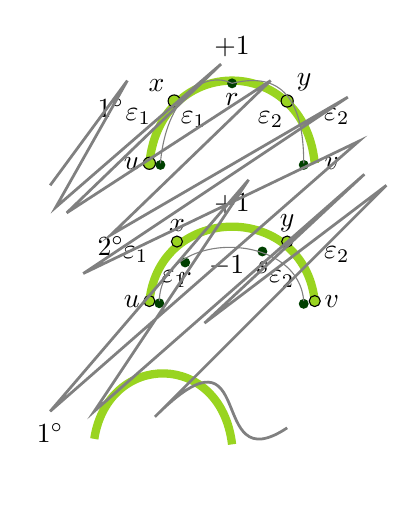
\begin{tikzpicture}[scale=.7]
\node at (-.7,1) {$1^\circ$};
\draw[yellow!60!green,line width=3pt] (0,0)..controls (.2,2) and (2.8,2)..(3,0);
\foreach \p in {(0,0),(.45,1.13),(2.5,1.13)}{\fill[yellow!60!green] \p circle(.11); \draw \p circle(.11);}
\fill[green!25!black] (1.5,1.45) circle(.09) (.2,-.03) circle(.09) (2.8,-.03) circle(.09);
\node[left] at (0,0) {$u$}; \node[above left] at (.45,1.13) {$x$}; \node[above right] at (2.5,1.13) {$y$}; \node[right] at (3,0) {$v$};
\node[below] at (1.5,1.45) {$r$}; \node[above] at (1.5,1.75) {$+1$};
\draw[gray] (.2,0)..controls (.3,1.2) and (1,1.7)..(1.5,1.45)..controls (2.5,1.7) and (2.8,1)..(2.8,0);
\node at (.8,.8) {$\varepsilon_1$}; \node at (2.2,.8) {$\varepsilon_2$}; \node at (-.2,.85) {$\varepsilon_1$}; \node at (3.4,.85) {$\varepsilon_2$};
\begin{scope}[shift={(0,-2.5)}]
\node at (-.7,1) {$2^\circ$};
\draw[yellow!60!green,line width=3pt] (0,0)..controls (.2,1.8) and (2.8,1.8)..(3,0);
\foreach \p in {(0,0),(.5,1.08),(2.5,1.08),(3,0)}{\fill[yellow!60!green] \p circle(.1); \draw \p circle(.1);}
\foreach \p in {(.18,-.04),(.65,.7),(2.05,.9),(2.8,-.05)}{\fill[green!25!black] \p circle(.09);}
\node[left] at (0,0) {$u$}; \node[above] at (.5,1.08) {$x$}; \node[above] at (2.5,1.08) {$y$}; \node[right] at (3,0) {$v$}; \node[below] at (.65,.7) {$r$}; \node[below] at (2.05,.9) {$s$};
\node at (1.4,.65) {$-1$}; \node[above] at (1.5,1.4) {$+1$};
\draw[gray] (.18,0)..controls (.2,1.3) and (2.7,1.3)..(2.8,0);
\node at (.45,.4) {$\varepsilon_1$}; \node at (2.4,.4) {$\varepsilon_2$}; \node at (-.25,.85) {$\varepsilon_1$}; \node at (3.4,.85) {$\varepsilon_2$};
\end{scope}
\node at (-1.8,-4.9) {$1^\circ$};
\draw[yellow!60!green,line width=3pt] (-1,-5)..controls (-.75,-3.4) and (1.3,-3.4)..(1.5,-5.1);
\draw[gray,line width=1pt] (-1.8,-.4)--(-.4,1.5)--(-1.7,-.8)--(1.3,1.8)--(-1.5,-.9)--(2.2,1.5)--(-.7,-1.3)--(3.6,1.2)--(-1.2,-2)--(3.8,.4)--(-1.8,-4.5)--(1.8,-.3)--(-1,-4.5)--(3.9,-.2)--(1,-2.9)--(4.3,-.4)--(.1,-4.6)..controls (2,-2.7) and (1,-5.8)..(2.5,-4.8);
\end{tikzpicture}}}

% E: drawing|right lower-middle, revised case 1|u x r y v arch signs epsilon1 epsilon2
\figure{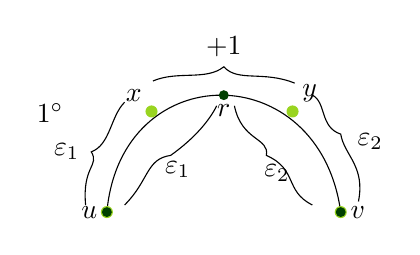
\begin{tikzpicture}[scale=.9]
\node at (-.8,1.4) {$1^\circ$};
\draw (0,0)..controls (.2,2.2) and (3,2.2)..(3.3,0);
\foreach \p in {(0,0),(.63,1.42),(2.62,1.42),(3.3,0)}{\fill[yellow!60!green] \p circle(.085);}
\foreach \p in {(0,0),(1.65,1.65),(3.3,0)}{\fill[green!25!black] \p circle(.07);}
\node[left] at (0,0) {$u$}; \node[above left] at (.63,1.42) {$x$}; \node[above right] at (2.62,1.42) {$y$}; \node[right] at (3.3,0) {$v$}; \node[below] at (1.65,1.65) {$r$};
\draw (.65,1.85)..controls (1,2) and (1.4,1.85)..(1.65,2.05)..controls (1.85,1.83) and (2.2,2)..(2.65,1.82);
\node[above] at (1.65,2.05) {$+1$};
\draw (-.3,.1)..controls (-.35,.65) and (-.1,.65)..(-.22,.85)..controls (.05,.95) and (.05,1.35)..(.25,1.55);
\node[left] at (-.25,.85) {$\varepsilon_1$};
\draw (2.9,1.65)..controls (3.1,1.55) and (3,1.2)..(3.3,1.1)..controls (3.35,.8) and (3.65,.65)..(3.55,.15);
\node[right] at (3.4,1) {$\varepsilon_2$};
\draw (.25,.1)..controls (.6,.45) and (.55,.75)..(.9,.8)..controls (1.25,1.05) and (1.45,1.3)..(1.55,1.5);
\node at (1,.6) {$\varepsilon_1$};
\draw (1.8,1.5)..controls (1.9,1) and (2.3,1.05)..(2.25,.8)..controls (2.7,.6) and (2.5,.3)..(2.9,.1);
\node at (2.4,.55) {$\varepsilon_2$};
\end{tikzpicture}}

% E: drawing|right lower, revised case 2|u r x s y v plus one minus one
\figure{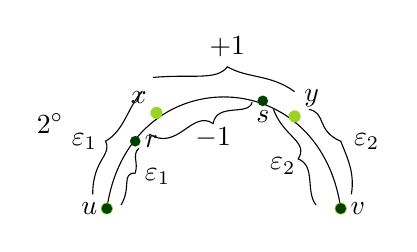
\begin{tikzpicture}[scale=.9]
\node at (-.8,1.2) {$2^\circ$};
\draw (0,0)..controls (.3,2.1) and (3,2.1)..(3.3,0);
\foreach \p in {(0,0),(.7,1.35),(2.65,1.3),(3.3,0)}{\fill[yellow!60!green] \p circle(.085);}
\foreach \p in {(0,0),(.4,.95),(2.2,1.52),(3.3,0)}{\fill[green!25!black] \p circle(.075);}
\node[left] at (0,0) {$u$}; \node[above left] at (.7,1.35) {$x$}; \node[above right] at (2.65,1.3) {$y$}; \node[right] at (3.3,0) {$v$}; \node[right] at (.4,.95) {$r$}; \node[below] at (2.2,1.52) {$s$};
\draw (.65,1.85)..controls (1.2,1.9) and (1.55,1.8)..(1.7,2)..controls (2,1.83) and (2.3,1.9)..(2.65,1.65);
\node[above] at (1.7,2) {$+1$};
\draw (.6,1.05)..controls (1,.8) and (1.2,1.4)..(1.5,1.2)..controls (1.55,1.5) and (2,1.3)..(2.05,1.5);
\node at (1.5,1) {$-1$};
\draw (-.2,.2)..controls (-.2,.7) and (.08,.75)..(-.02,.95)..controls (.25,1.1) and (.3,1.45)..(.5,1.65);
\node[left] at (0,.95) {$\varepsilon_1$};
\draw (.2,.05)..controls (.35,.3) and (.2,.5)..(.4,.5)..controls (.45,.65) and (.35,.75)..(.45,.85);
\node[right] at (.4,.45) {$\varepsilon_1$};
\draw (2.35,1.4)..controls (2.5,1) and (2.85,.95)..(2.7,.7)..controls (2.95,.6) and (2.8,.25)..(2.95,.05);
\node[left] at (2.8,.6) {$\varepsilon_2$};
\draw (2.85,1.4)..controls (3.1,1.35) and (2.95,1.1)..(3.3,.95)..controls (3.4,.7) and (3.5,.5)..(3.45,.2);
\node[right] at (3.35,.95) {$\varepsilon_2$};
\end{tikzpicture}}

% E: drawing|bottom right, revised case 3|arch with three dark interior vertices
\figure{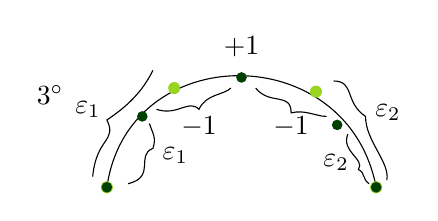
\begin{tikzpicture}[scale=.9]
\node at (-.8,1.3) {$3^\circ$};
\draw (0,0)..controls (.3,2.1) and (3.4,2.1)..(3.8,0);
\foreach \p in {(0,0),(.95,1.4),(2.95,1.35),(3.8,0)}{\fill[yellow!60!green] \p circle(.085);}
\foreach \p in {(0,0),(.5,1),(1.9,1.55),(3.25,.88),(3.8,0)}{\fill[green!25!black] \p circle(.075);}
\node[above] at (1.9,1.7) {$+1$};
\draw (.7,1.1)..controls (1,1) and (1.15,1.25)..(1.3,1.1)..controls (1.4,1.32) and (1.65,1.3)..(1.75,1.4);
\draw (2.1,1.4)..controls (2.3,1.15) and (2.6,1.35)..(2.6,1.05)..controls (2.8,1.1) and (2.95,1)..(3.1,1);
\node at (1.3,.85) {$-1$}; \node at (2.6,.85) {$-1$};
\draw (-.2,.15)..controls (-.15,.7) and (.15,.65)..(0,.95)..controls (.3,1.15) and (.5,1.35)..(.65,1.65);
\node[left] at (.05,1.1) {$\varepsilon_1$};
\draw (.3,.05)..controls (.7,.15) and (.4,.45)..(.65,.55)..controls (.7,.7) and (.65,.75)..(.6,.9);
\node[right] at (.65,.45) {$\varepsilon_1$};
\draw (3.4,.75)..controls (3.3,.5) and (3.65,.4)..(3.55,.25)..controls (3.65,.2) and (3.6,.12)..(3.7,.05);
\node[left] at (3.55,.35) {$\varepsilon_2$};
\draw (3.2,1.5)..controls (3.5,1.5) and (3.35,1.2)..(3.65,1)..controls (3.65,.65) and (4,.35)..(3.95,.1);
\node[right] at (3.65,1.05) {$\varepsilon_2$};
\end{tikzpicture}}
\mspage{53}
